%%%%%%%% ICML 2022 EXAMPLE LATEX SUBMISSION FILE %%%%%%%%%%%%%%%%%

\documentclass[nohyperref]{article}

% Recommended, but optional, packages for figures and better typesetting:
\usepackage{microtype}
\usepackage{graphicx}
\usepackage{subfigure}
\usepackage{booktabs} % for professional tables

% hyperref makes hyperlinks in the resulting PDF.
% If your build breaks (sometimes temporarily if a hyperlink spans a page)
% please comment out the following usepackage line and replace
% \usepackage{icml2022} with \usepackage[nohyperref]{icml2022} above.
\usepackage{hyperref}


% Attempt to make hyperref and algorithmic work together better:
\newcommand{\theHalgorithm}{\arabic{algorithm}}

% Use the following line for the initial blind version submitted for review:
\usepackage{icml2022}

% If accepted, instead use the following line for the camera-ready submission:
% \usepackage[accepted]{icml2022}

% For theorems and such
\usepackage{amsmath}
\usepackage{amssymb}
\usepackage{mathtools}
\usepackage{amsthm}

% if you use cleveref..
\usepackage[capitalize,noabbrev]{cleveref}

%%%%%%%%%%%%%%%%%%%%%%%%%%%%%%%%
% THEOREMS
%%%%%%%%%%%%%%%%%%%%%%%%%%%%%%%%
\theoremstyle{plain}
\newtheorem{theorem}{Theorem}[section]
\newtheorem{proposition}[theorem]{Proposition}
\newtheorem{lemma}[theorem]{Lemma}
\newtheorem{corollary}[theorem]{Corollary}
\theoremstyle{definition}
\newtheorem{definition}[theorem]{Definition}
\newtheorem{assumption}[theorem]{Assumption}
\theoremstyle{remark}
\newtheorem{remark}[theorem]{Remark}

% Todonotes is useful during development; simply uncomment the next line
%    and comment out the line below the next line to turn off comments
%\usepackage[disable,textsize=tiny]{todonotes}
\usepackage[textsize=tiny]{todonotes}


% The \icmltitle you define below is probably too long as a header.
% Therefore, a short form for the running title is supplied here:
\icmltitlerunning{Disentangling Emergent Groups}

\begin{document}

\twocolumn[
\icmltitle{Disentangling Emergent Groups}

% It is OKAY to include author information, even for blind
% submissions: the style file will automatically remove it for you
% unless you've provided the [accepted] option to the icml2022
% package.

% List of affiliations: The first argument should be a (short)
% identifier you will use later to specify author affiliations
% Academic affiliations should list Department, University, City, Region, Country
% Industry affiliations should list Company, City, Region, Country

% You can specify symbols, otherwise they are numbered in order.
% Ideally, you should not use this facility. Affiliations will be numbered
% in order of appearance and this is the preferred way.
% \icmlsetsymbol{equal}{*}

\begin{icmlauthorlist}
\icmlauthor{Dan Andrei Iliescu}{cam}
\icmlauthor{Damon J Wischik}{cam}
\end{icmlauthorlist}

\icmlaffiliation{cam}{Department of Computer Science, University of Cambridge, UK}

\icmlcorrespondingauthor{Dan Andrei Iliescu}{dai24@cam.ac.uk}

% You may provide any keywords that you
% find helpful for describing your paper; these are used to populate
% the "keywords" metadata in the PDF but will not be shown in the document
\icmlkeywords{Machine Learning, ICML}

\vskip 0.3in
]

% this must go after the closing bracket ] following \twocolumn[ ...

% This command actually creates the footnote in the first column
% listing the affiliations and the copyright notice.
% The command takes one argument, which is text to display at the start of the footnote.
% The \icmlEqualContribution command is standard text for equal contribution.
% Remove it (just {}) if you do not need this facility.

%\printAffiliationsAndNotice{}  % leave blank if no need to mention equal contribution
\printAffiliationsAndNotice{\icmlEqualContribution} % otherwise use the standard text.

\begin{abstract}
Group-instance disentanglement is the problem of learning separate representations for within-group and across-group variation.  In our work,  we propose the Context-Aware Variational Autoencoder (CxVAE), a method that can perform group-instance disentanglement on data with ``emergent'' groups (i.e.  data where the group and instance variables cannot be inferred from a single datapoint). First,  we introduce a simple synthetic dataset to show that current state-of-the-art methods based on the Group VAE fail to learn disentangled representations on datasets with ``emergent groups''; Next, we present a modified model that 1) infers the instance variable conditionally on the group variable, 2) has a more expressive group encoder, 3) optimizes a regularization objective that encourages independence between the instance variable and the grouping. Finally, we show empirically the impact of each modification with respect to holdout data likelihood, unsupervised translation, and other disentanglement metrics.
\end{abstract}

\section{Introduction}
\label{intro}

\begin{figure}[t]
    \vskip 0.2in
    \begin{center}
    \centerline{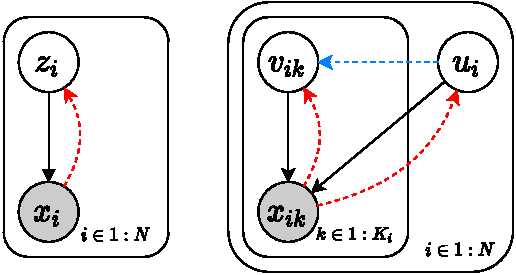
\includegraphics[width=\columnwidth]{files/bayes_net.pdf}}
    \caption{Probabilistic graphical model of the VAE (left) and the GVAE (right). The dotted arrows depict the variational latent posterior. \textbf{The blue arrow shows a dependency which is absent from existing methods but present in our proposed model.}}
    \label{bayes-net}
    \end{center}
    \vskip -0.2in
\end{figure}

The goal of group-instance disentanglement is to learn a representation network that transforms grouped observations (e.g. images grouped by author,  temperature readings grouped by weather station,  etc) into two latent variables,  \textit{group} and \textit{instance}.  The group variable should capture the information which distinguishes one group from another, but exclude the information which can identify a particular observation within the group. The instance variable should do vice-versa: capture all of the individual information, but none of the group information.

All the current state-of-the-art approaches to group-instance disentanglement \citep{Bouchacourt2018MultiLevelVA,Hosoya2019GroupbasedLO,Shu2020Weakly, Chen2020WeaklySD,Locatello2020WeaklySupervisedDW} follow the Variational Autoencoder framework \citep{Kingma2014AutoEncodingVB,JimenezRezende2014StochasticBA} whereby a generative model mapping latent variables (group and instance) to data observations is trained using variational inference. We call this family of models the Group Variational Autoencoder (GVAE). These methods vary in how they define the variational latent posterior and any additional regularization objectives they might have.

We believe that GVAE has the potential to advance many scientific fields where analysing the causal factors of grouped data is essential, including medicine \citep{Liang1986LongitudinalDA}, biology \citep{Quinn2002ExperimentalDA} and psychology \citep{Schafer2002MissingDO}. That analysis is typically performed using mixed-effects models \citep{Pinheiro2001MixedEffectsMI}, which decompose the data variation into random-effects (group variables) and individual error terms (instance variables). However, these parameters can only be estimated efficiently in very simple models. By contrast, the GVAE offers a highly expressive mixed-effects model (the decoder) and an inbuilt inference network (the encoder).

In order to learn useful disentangled representations for these problems,  the GVAE has to capture the joint distribution between the group and instance variables conditioned on the data. In other words,  the representation network must be able to distinguish between two identical observations coming from different groups, thus encoding them with different instance variables.  We call data groups of this kind ``emergent'', because the group and instance variables are emergent properties of the group as a whole, rather than any individual observation. 

Emergent groups are very common, occurring in datasets where the latent variables cannot be accurately inferred from a single observation. For example, in the context of soybean plant growth \citep{Davidian1995NonlinearMF}, it is impossible to deduce the age (instance) of a plant based solely on its leaf weight (observation) without also knowing its genotype (group). 

Unfortunately,  the current state-of-the-art methods fail to learn disentangled representations on emergent groups.We show this empirically by creating a simple dataset of student exam scores grouped by school. The groups in this dataset are emergent, because the instance variable captures the score of a student in relation to the distribution of scores at their school. Instead of disentangling, the existing methods mostly forego the group variable and use the instance variable to encode the variation across groups. The main

In order to tackle this challenge, we propose a new GVAE model with several novel modifications. The main novelty is an instance encoder conditional on the previously inferred group variable, which enables the variational latent posterior to match the generative latent posterior.  Additionally, we use an expressive Deep Set network \citep{Zaheer2017DeepS} to infer the group variable more accurately, and also design a novel regularization objective that encourages independence between the inferred instance variable and the data group. 

Our work comprises the following contributions:
\begin{enumerate}
    \item We formalize the notion of ``emergent'' groups and create a simple synthetic dataset on which the current GVAE methods fail to learn disentangled representations.
    \item We propose a new model, called the Context-Aware Variational Autoencoder (CxVAE) which can learn disentangled representations on emergent groups.
    \item We perform extensive evaluation showing that our model outperforms the existing methods in holdout-data log-likelihood, unsupervised translation, and ground-truth factor prediction.
    \item We perform an ablation study showing the relative performance gain of each modification to the GVAE.
\end{enumerate}

\section{Generative Group-Instance}

The Group Variational Autoencoder \citep{Bouchacourt2018MultiLevelVA,Hosoya2019GroupbasedLO} is a family of models that use two latent variables to represent grouped data: one that captures the variation within groups, and one for the variation across groups.

Assume a dataset of the form $\{x_{ik}\}_{i \in 1:N, ~k \in 1:K_i}$ where $N$ is the number of groups and $K_i$ is the number of observations in group $i$. GVAE defines a generative model that maps a $\mathcal{N} (0,1)$ group latent variable $u_i$ and a $\mathcal{N} (0,1)$ instance latent variable $v_{ik}$ to a given data observation $x_{ik}$. In other words, the likelihood of a group is:

$$p(\mathbf{x}) = \mathbb{E}_{p(u)}  \prod_{k=1}^{K} \mathbb{E}_{p(v_{k})} ~ [p(x_{k} | u, v_{k})]$$

We omit the index of the group $i$ for notational simplicity, since the groups are independent and identically distributed.

\subsection{Variational Inference}

Because the exact likelihood is intractable, the Variational Autodencoder \citep{Kingma2014AutoEncodingVB,JimenezRezende2014StochasticBA} performs optimization by introducting a variational latent posterior $q(u, \mathbf{v} | \mathbf{x})$ and maximizing the Evidence Lower Bound \citep{Jordan2004AnIT}:

$$\log p(\mathbf{x}) \geq \mathbb{E}_{q(u, \mathbf{v} | \mathbf{x})} [\log p(\mathbf{x} | u, \mathbf{v})] - \mathrm{KL} [q(u, \mathbf{v} | \mathbf{x}) || p(u, \mathbf{v})]$$

\textit{The models in the GVAE family use a class of variational distributions that assume independence between the latent variables in a group when conditioned on the data.}

$$q(u, \mathbf{v} | \mathbf{x}) = q(u | \mathbf{x}) \prod_{k=1}^K q(v_k | x_k)$$

In our work, we show that this assumption hinders disentanglement when the generative model is entangled.

\subsection{Group Encoder}

The variational group posterior is realised as normal density with $\mu, \Sigma$ computed with an encoder network. The way to implement the encoder network is not obvious, since the number of inputs $K$ varies across groups. \citet{Hosoya2019GroupbasedLO} encode separately each observation in the group using the same encoder $E_u$ to produce $\mu_k, \Sigma_k$ and then averages the outputs.

$$\mu = \frac{1}{N} \sum_{k=1}^K \mu_k, ~ \Sigma = \frac{1}{N} \sum_{k=1}^K \Sigma_k$$

\citet{Bouchacourt2018MultiLevelVA} also encode each observation individually and then accumulate the evidence through a product of normal densities, computed using the following equations:

$$\Sigma^{-1} = \sum_{k=1}^K \Sigma_k^{-1}, ~ \mu^T \Sigma^{-1} = \sum_{k=1}^K \mu_k^T \Sigma_k^{-1}$$

They justify that such a product of normals produces a valid evidence accumulation using the following result:

$$q(u | \mathbf{x}) \propto \prod_{k=1}^K q(u | x_k)$$

However, the above is not a universal property, since

\begin{align}
    \begin{split}
        q(u | \mathbf{x}) = &\frac{\prod_{k=1}^K q(x_k)}{q(\mathbf{x})} \frac{1}{q(u)^{K-1}} \prod_{k=1}^K q(u | x_k) \\ &\propto \frac{1}{q(u)^{K-1}} \prod_{k=1}^K q(u | x_k)
    \end{split}
\end{align}

In fact, by using a product of normals to accumulate evidence, the authors implicitly assume that the marginal distribution of the inferred group variable is a uniform. This has the effect of sampling $u$ values which are less representative of the current group and more skewed towards the marginal distribution of $u$.

In our work, we propose a more general approach to encoding $u$ by using a Deep Sets  network \citep{Zaheer2017DeepS} to encode the whole set of observations instead of encoding each observation separately.

\subsection{Regularization}

In certain cases, the model might learn to encode both kinds of variation (within- and across-group) in the instance variable, effectively turning the model into a standard VAE. In this eventuality, the group variable becomes irrelevant and disentanglement is not achieved.

Such behaviour has been identified by \citet{Hosoya2019GroupbasedLO} and \citet{Nmeth2020AdversarialDW} to occur when the instance code too high-dimensional, the instance encoder too expressive, or group sizes too small. One solution is to limit the dimensionality of the instance code \citep{Hosoya2019GroupbasedLO}, with the downside of hindering the overall model performance. 

As a more targeted solution, \citet{Hosoya2019GroupbasedLO} propose an adversarial loss minimizing the mutual information between an observation and the instance variable inferred from the other observations in the group:

$$I_{r} (x, v) = \mathrm{KL} [r(x, v) || r(x) r(v)]$$

where $r(x, v) = r(v | x) r(x)$ is the joint distribution of an observation and the instance variable inferred from any of the other observations in the group and 

$$r(v | x_k) = \frac{1}{K - 1} \sum_{l=1, ~ l \neq k}^K q(v | x_l)$$

The mutual information is approximated empirically using the results of \citet{Belghazi2018MutualIN}.

\begin{align}
\begin{split}
I_{r} (x, v) \approx \max_{T} ~ &\mathbb{E}_{r(x, v)} [T(x, v)] \\ &- \log \mathbb{E}_{r(x)r(v)} [\exp T(x, v)] 
\end{split}
\end{align}

$T$ is a neural network and the expectation terms are computed by sampling.

\begin{itemize}
    \item To sample $r(x, v)$, first choose a group $i$, then choose two instances from that group $k, l \in K_i$. $x$ will be the observation $x_{ik}$ and $v$ will be sampled from $q(v | x_{il})$.
    \item To sample $r(x)r(v)$, choose two groups $i, j$ and two instances in each group $k \in K_i, l \in K_j$. Take $x_{ik}$ for $x$ and sample $q(v | x_{jl})$.
\end{itemize}

In our view, this method has the following limitation: Even when the instance variable does contain group information, the value of $I_{r} (x, v)$ might still be small, because it might be difficult to ascertain the group based on one single observation $x$. In our work, we propose a modification to this regularization term such that the network $T$ takes as input all the observations in the group instead of only one.

\section{Entangled Group and Instance Variables}

We call the group and instance variables \textit{entangled} when they are not independent conditioned on the data $p(u, v | x) \neq p(u | x) p(v | x)$. A useful heuristic for establishing whether the variables are entangled is to ask ``Does knowing the group variable for an observation influence my belief about its instance variable?''

This property of the generative model is present in many machine learning tasks, such as collaborative filtering, 3D novel view synthesis. For example, in the context of the Netflix Challenge, where the task was to predict what score a user would give to a new film, one cannot infer what film is associated with a given score without also knowing the user.

\textit{Strictly speaking, most real-world models are entangled. However, in many cases, the mutual information between the group and instance variable, conditioned on the observation, is negligible. For example, in handwritten digit recognition, one can infer the digit value depicted in an image without knowing the author.}

In this paper, we claim that the current methods in the GVAE family do not perform well in tasks where the group and instance variables are entangled.

\subsection{Exam-Scores Problem}

\begin{figure}[ht]
    \vskip 0.2in
    \begin{center}
    \centerline{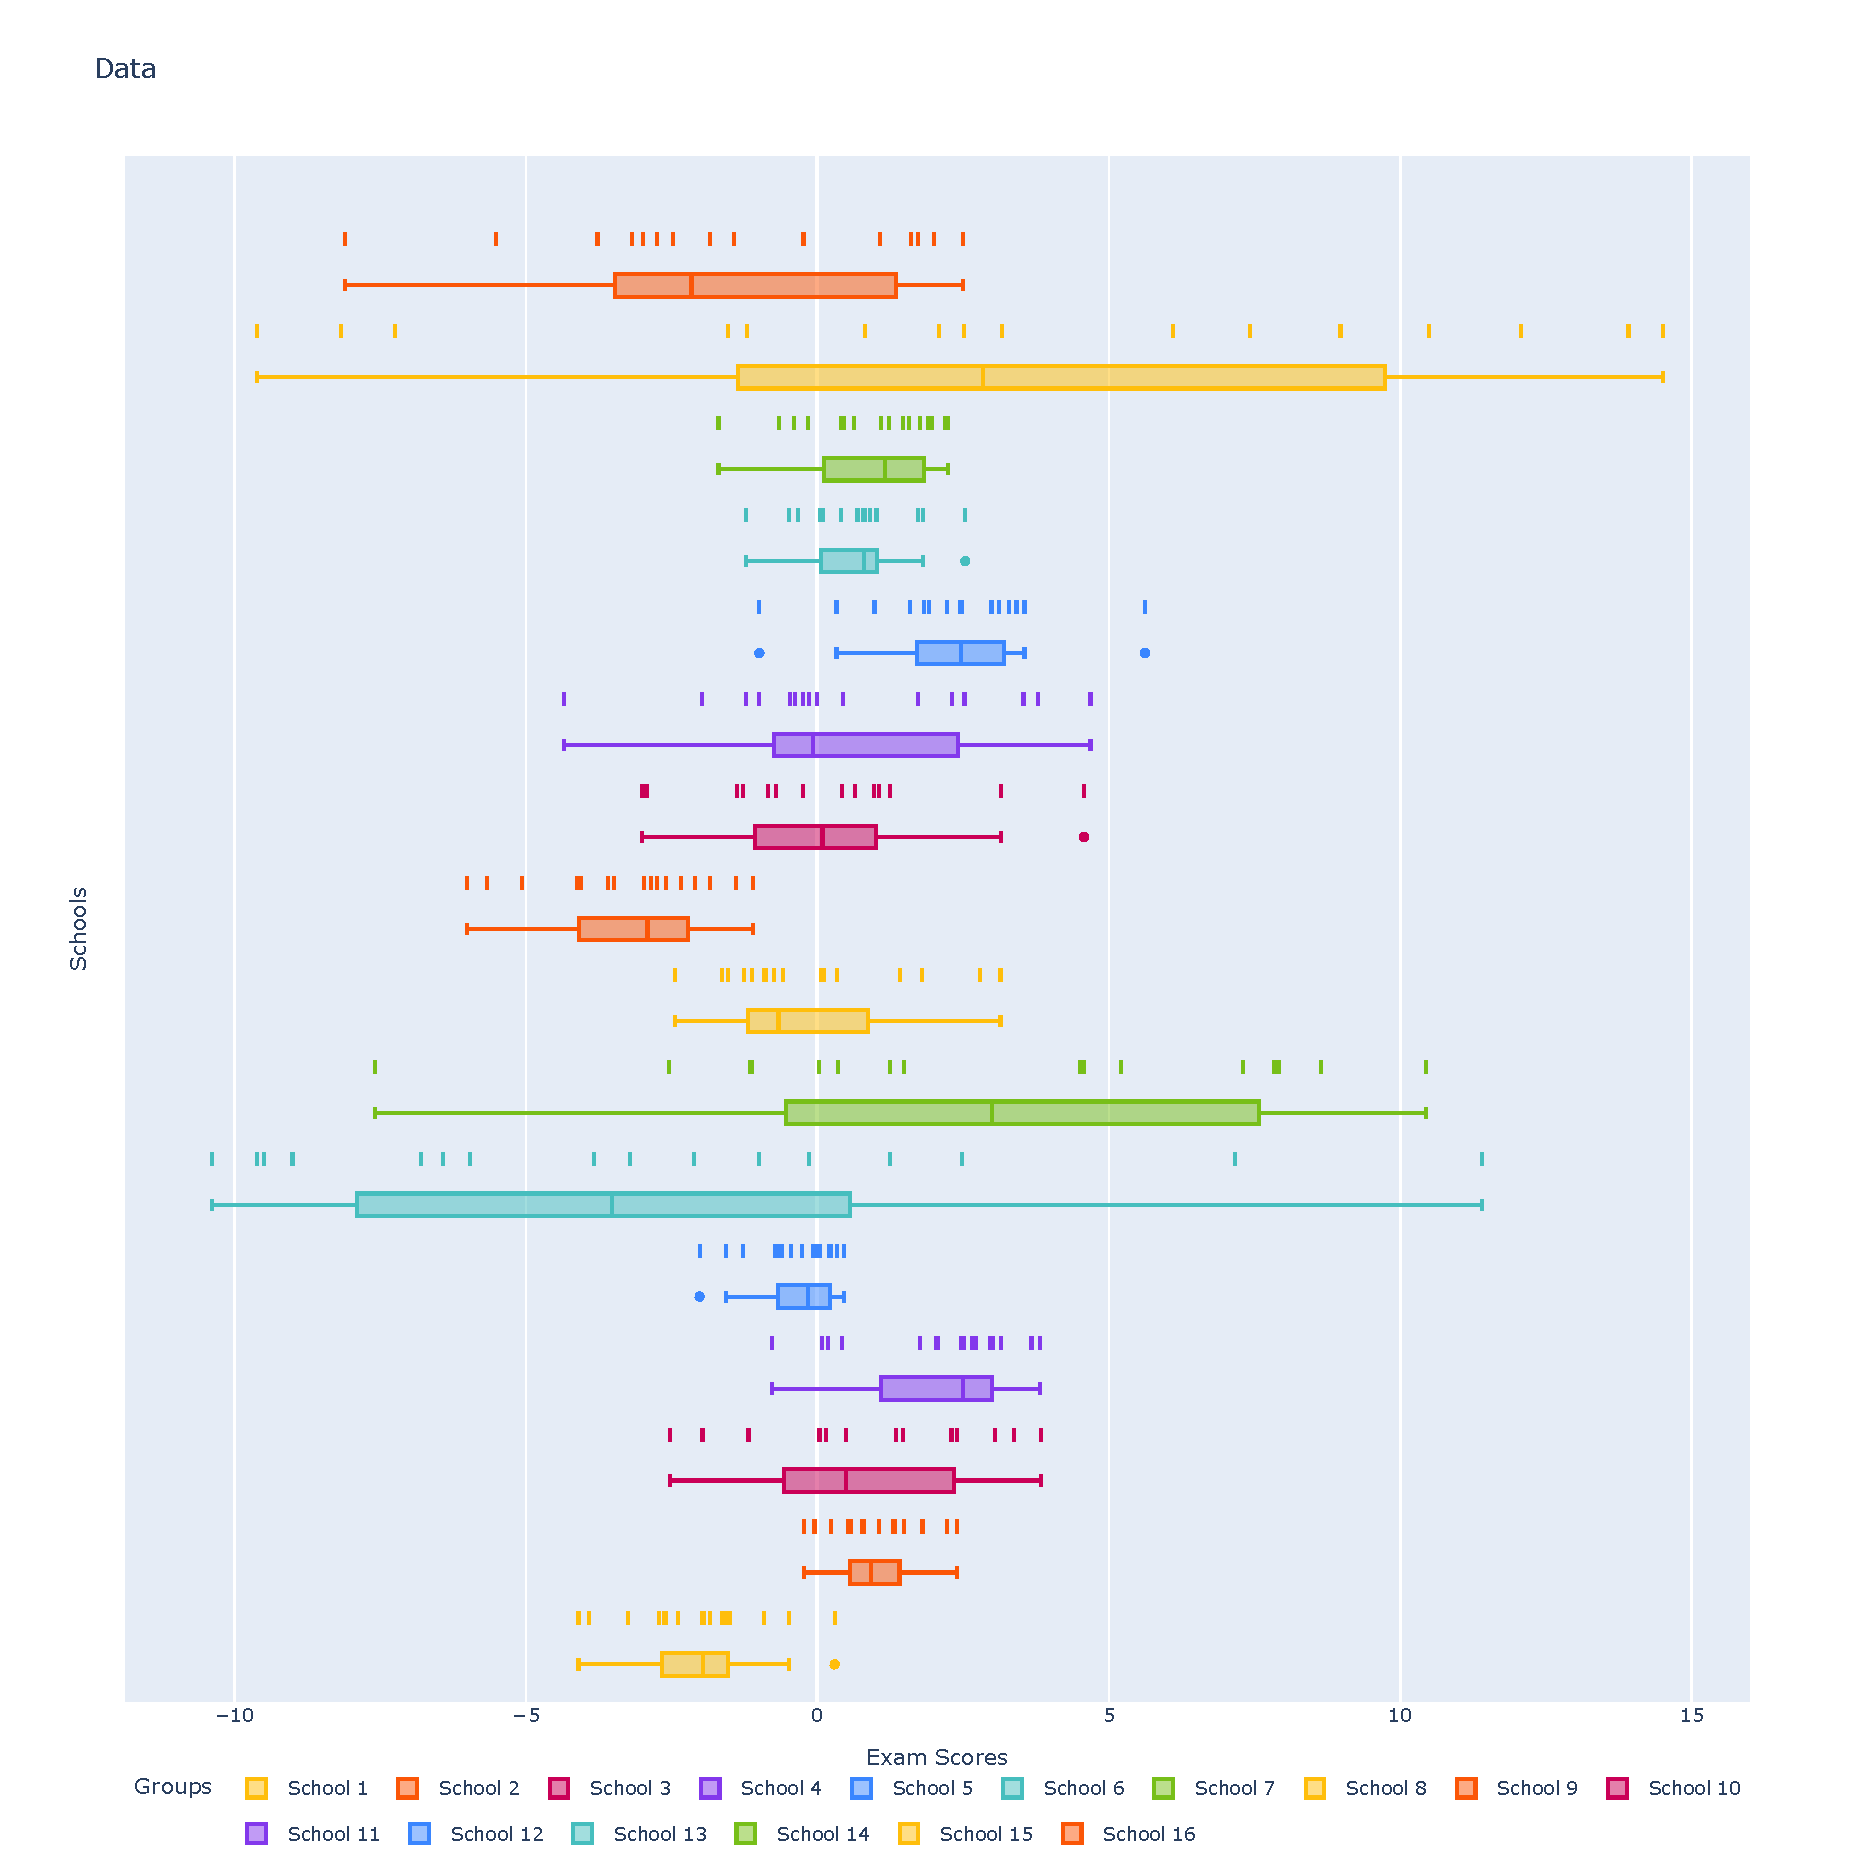
\includegraphics[width=\columnwidth]{files/data.pdf}}
    \caption{\textbf{Normalized exam scores of individual students grouped by school.}}
    \label{exam-score}
    \end{center}
    \vskip -0.2in
\end{figure}

Suppose we wanted to model the exam scores of students from different schools. Our model must separate the school-level effect (the group factor) from the student-level effect (the instance factor). We define the following generative model:

$$x_{ik} = 2 ~ \mu_i +  (\sigma^2_i + 1) v_{ik} + \epsilon_{ik}, ~ i \in 1:N, ~ k \in 1:K_i$$

where $x_{ij}$ is the student score, $u_i = (\mu_i, \sigma_i)$ is the school-level effect, $v_{ij}$ is the student-level effect, and $\epsilon_{ik}$ is a normally-distributed error term. We assume a $\mathcal{N} (0, 1)$ prior distribution for the latent variables.

We first sample the model to generate a dataset ($N = 32,768, ~ K_i \sim \mathrm{Poisson} (16) + 8$) and then use the same model as the generative model in our Variational Autoencoder, instead of a neural network. The figure below shows what the data looks like.

Looking at the data, it is easy to see that this model is entangled, because the relative performance $v$ of a student within their own school, given their absolute score $x$, depends on the distribution of scores within the school $u$.

\section{Context-Aware Variational Autoencoder (CxVAE)}

We propose a new model which can perform well on datasets generated from entangled group and instance variable. We call our model the Context-Aware Variational Autoencoder. Our model comprises the following changes with respect to the standard GVAE:

\begin{enumerate}
    \item The group encoder is implemented as a Deep Sets network \citep{Zaheer2017DeepS}. The encoder has the following form:
    $$\mu, \Sigma = E_u (\mathbf{x}) = E^B_u \left( \sum_{k=1}^K E^A_u (x_k)\right)$$
    where $E^A_u, E^B_u$ are two neural networks.
    \item The variational instance posterior is dependent on the inferred group variable:
    $$q(u, \mathbf{v} | \mathbf{x}) = q(u | \mathbf{x}) \prod_{k=1}^K q(v_k | x_k, u)$$
    In practice, our instance encoder takes as input a vector concatenating $x_k$ and $u$. This idea is not new, and has been used previously in sequence disentanglement \citep{Li2018DisentangledSA}. This allows the instance encoder to differentiate the between observations with similar values but which come from different groups.
    \item We propose a regularization objective similar to the one in \citet{Nmeth2020AdversarialDW}, but whereby we minimize \textit{the mutual information between one inferred instance variable and all the other observations in the group}. More precisely, our objective is to minimize $I_r (\mathbf{x}_{-k}, v_k)$ where $r(v_k | \mathbf{x}_{-k}) = q(v_k | x_k, u)$. Following the same approximation as in \citet{Nmeth2020AdversarialDW}, the objective takes the following form:
    \begin{align}
        \begin{split}
            I_{r} (\mathbf{x}_{-k}, v_k) &\approx \max_{T} ~ \mathbb{E}_{r(\mathbf{x}_{-k}, v_k)} [T(\mathbf{x}_{-k}, v_k)] \\ - \log &\mathbb{E}_{r(\mathbf{x}_{-k}) r(v_k)} [\exp T(\mathbf{x}_{-k}, v_k)]
        \end{split}
    \end{align}
    $T$ is implemented as a Deep Sets neural network for the observations, with the instance code concatenated in the middle:
    $$T(\mathbf{x}_{-k}, v_k) = T^\beta \left(v_k, \frac{1}{K} \sum_{l=1, ~ l \neq k}^K T^\alpha (x_l) \right)$$
    Again, the expectations are computed by sampling:
    \begin{itemize}
        \item To sample $r(x, v)$, first choose a group $i$, then choose one instance from that group $k \in K_i$. $\mathbf{x}_{i,-k}$ will be all the observations in the group apart from $k$, and $v_k$ will be sampled from $q(v | x_{ik})$.
        \item To sample $r(\mathbf{x}_{-k})r(v_k)$, choose two groups $i, j$ and two instances in each group $k \in K_i, ~ l \in K_j$. Take $\mathbf{x}_{i, -k}$ for $\mathbf{x}_{-k}$ and sample $q(v | x_{jl})$. 
    \end{itemize}
    
    This regularization objective also minimizes the mutual information between the inferred instance variables and the true data generating group variable, but uses as a proxy for the latter all but one of the observations in the group, instead of just one observation.
\end{enumerate}

\section{Measuring Disentanglement}

In the context of the GVAE family, disentanglement is a property of the variational latent posterior. The inferred group and instance variables are disentangled when they are maximally informative about the group and instance variables of the true data generating distribution. We assume this true model has the same factorization of the joint distribution as the generative model, but the parameters are unknown.

Therefore, we can use the mutual information between the true and inferred latents as a measure of disentanglement.

$$I(U^t; U^q) = \mathrm{KL} [\mathrm{Pr}_{U^q, U^t} || \mathrm{Pr}_{U^q} \mathrm{Pr}_{U^t}]$$
$$= \mathbb{E}_{U^q} \mathbb{E}_{U^t | U^q} \left[ \log \frac{\mathrm{Pr}_{U^t | U^q}}{\mathrm{Pr}_{U^t}} \right]$$
and since $\mathrm{Pr}_{U^t}$ does not depend on $q$
$$= \mathbb{E}_{U^q} \mathbb{E}_{U^t | U^q} [ \log \mathrm{Pr}_{U^t | U^q}] + \mathrm{const}$$

We estimate the density $\mathrm{Pr}_{U^t | U^q}$ by training a regression network to predict the value of $U^t$ given $U^q$. The mean-squared error of the prediction on the holdout set is a monotonic function of the mutual information with respect to changes in $q$.

\subsection{Unsupervised Translation}

\begin{figure}[ht]
    \vskip 0.2in
    \begin{center}
    \centerline{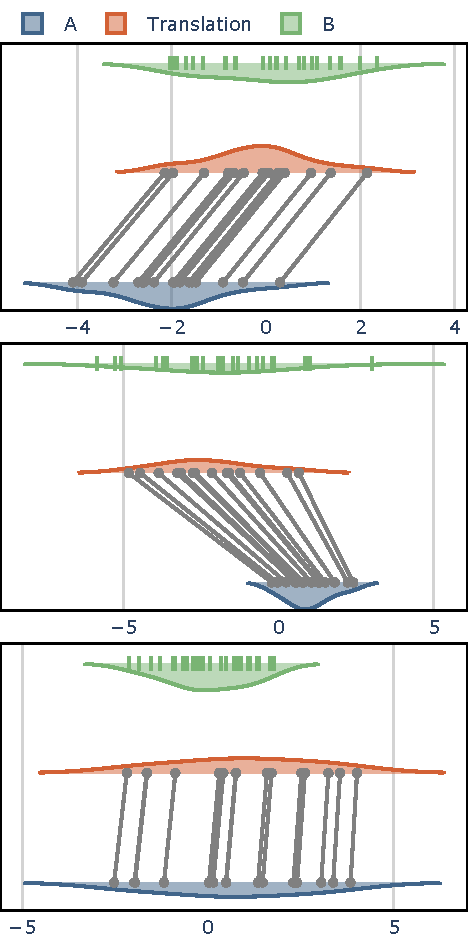
\includegraphics[width=\columnwidth]{files/data_trans.pdf}}
    \caption{\textbf{Example of translation on the Exam-Scores dataset.} The yellow and orange show the distributions of the source and target group, respectively. The red shows the distribution of the translated group. The grey lines show the translation of individual observations from the source to the target. We expect a good translation to have the translation lines uncrossed (the instance variable is preserved) and to have the same distribution as the target group (the group variable is changed).}
    \label{trans}
    \end{center}
    \vskip -0.2in
\end{figure}

Unsupervised translation is the process of transforming an observation by changing its group code while keeping its instance code fixed. This is a common downstream task for disentangled representations because it requires a clean separation between the group and instance representations \citep{Tenenbaum2000SeparatingSA}. Therefore, it can be used to quantify the quality of disentanglement.

Formally, let $i, j$ be the indices of the source and target group, respectively. Translation involves sampling a group of instance codes from the source group $q(\mathbf{v}_i | \mathbf{x}_i)$ and a group code from the target group $q(u_j | \mathbf{x}_j)$. Then, we generate the translated observations by combining each instance code with the group code $p(x'_{k} | u_j, \mathbf{v}_j)$.

We measure translation quality by taking the mean-squared error between the translation performed with each model and the ground-truth translation computed using the ground-truth factors and the true data-generating process.

\section{Evaluation}

\begin{figure}[ht]
    \vskip 0.2in
    \begin{center}
    \centerline{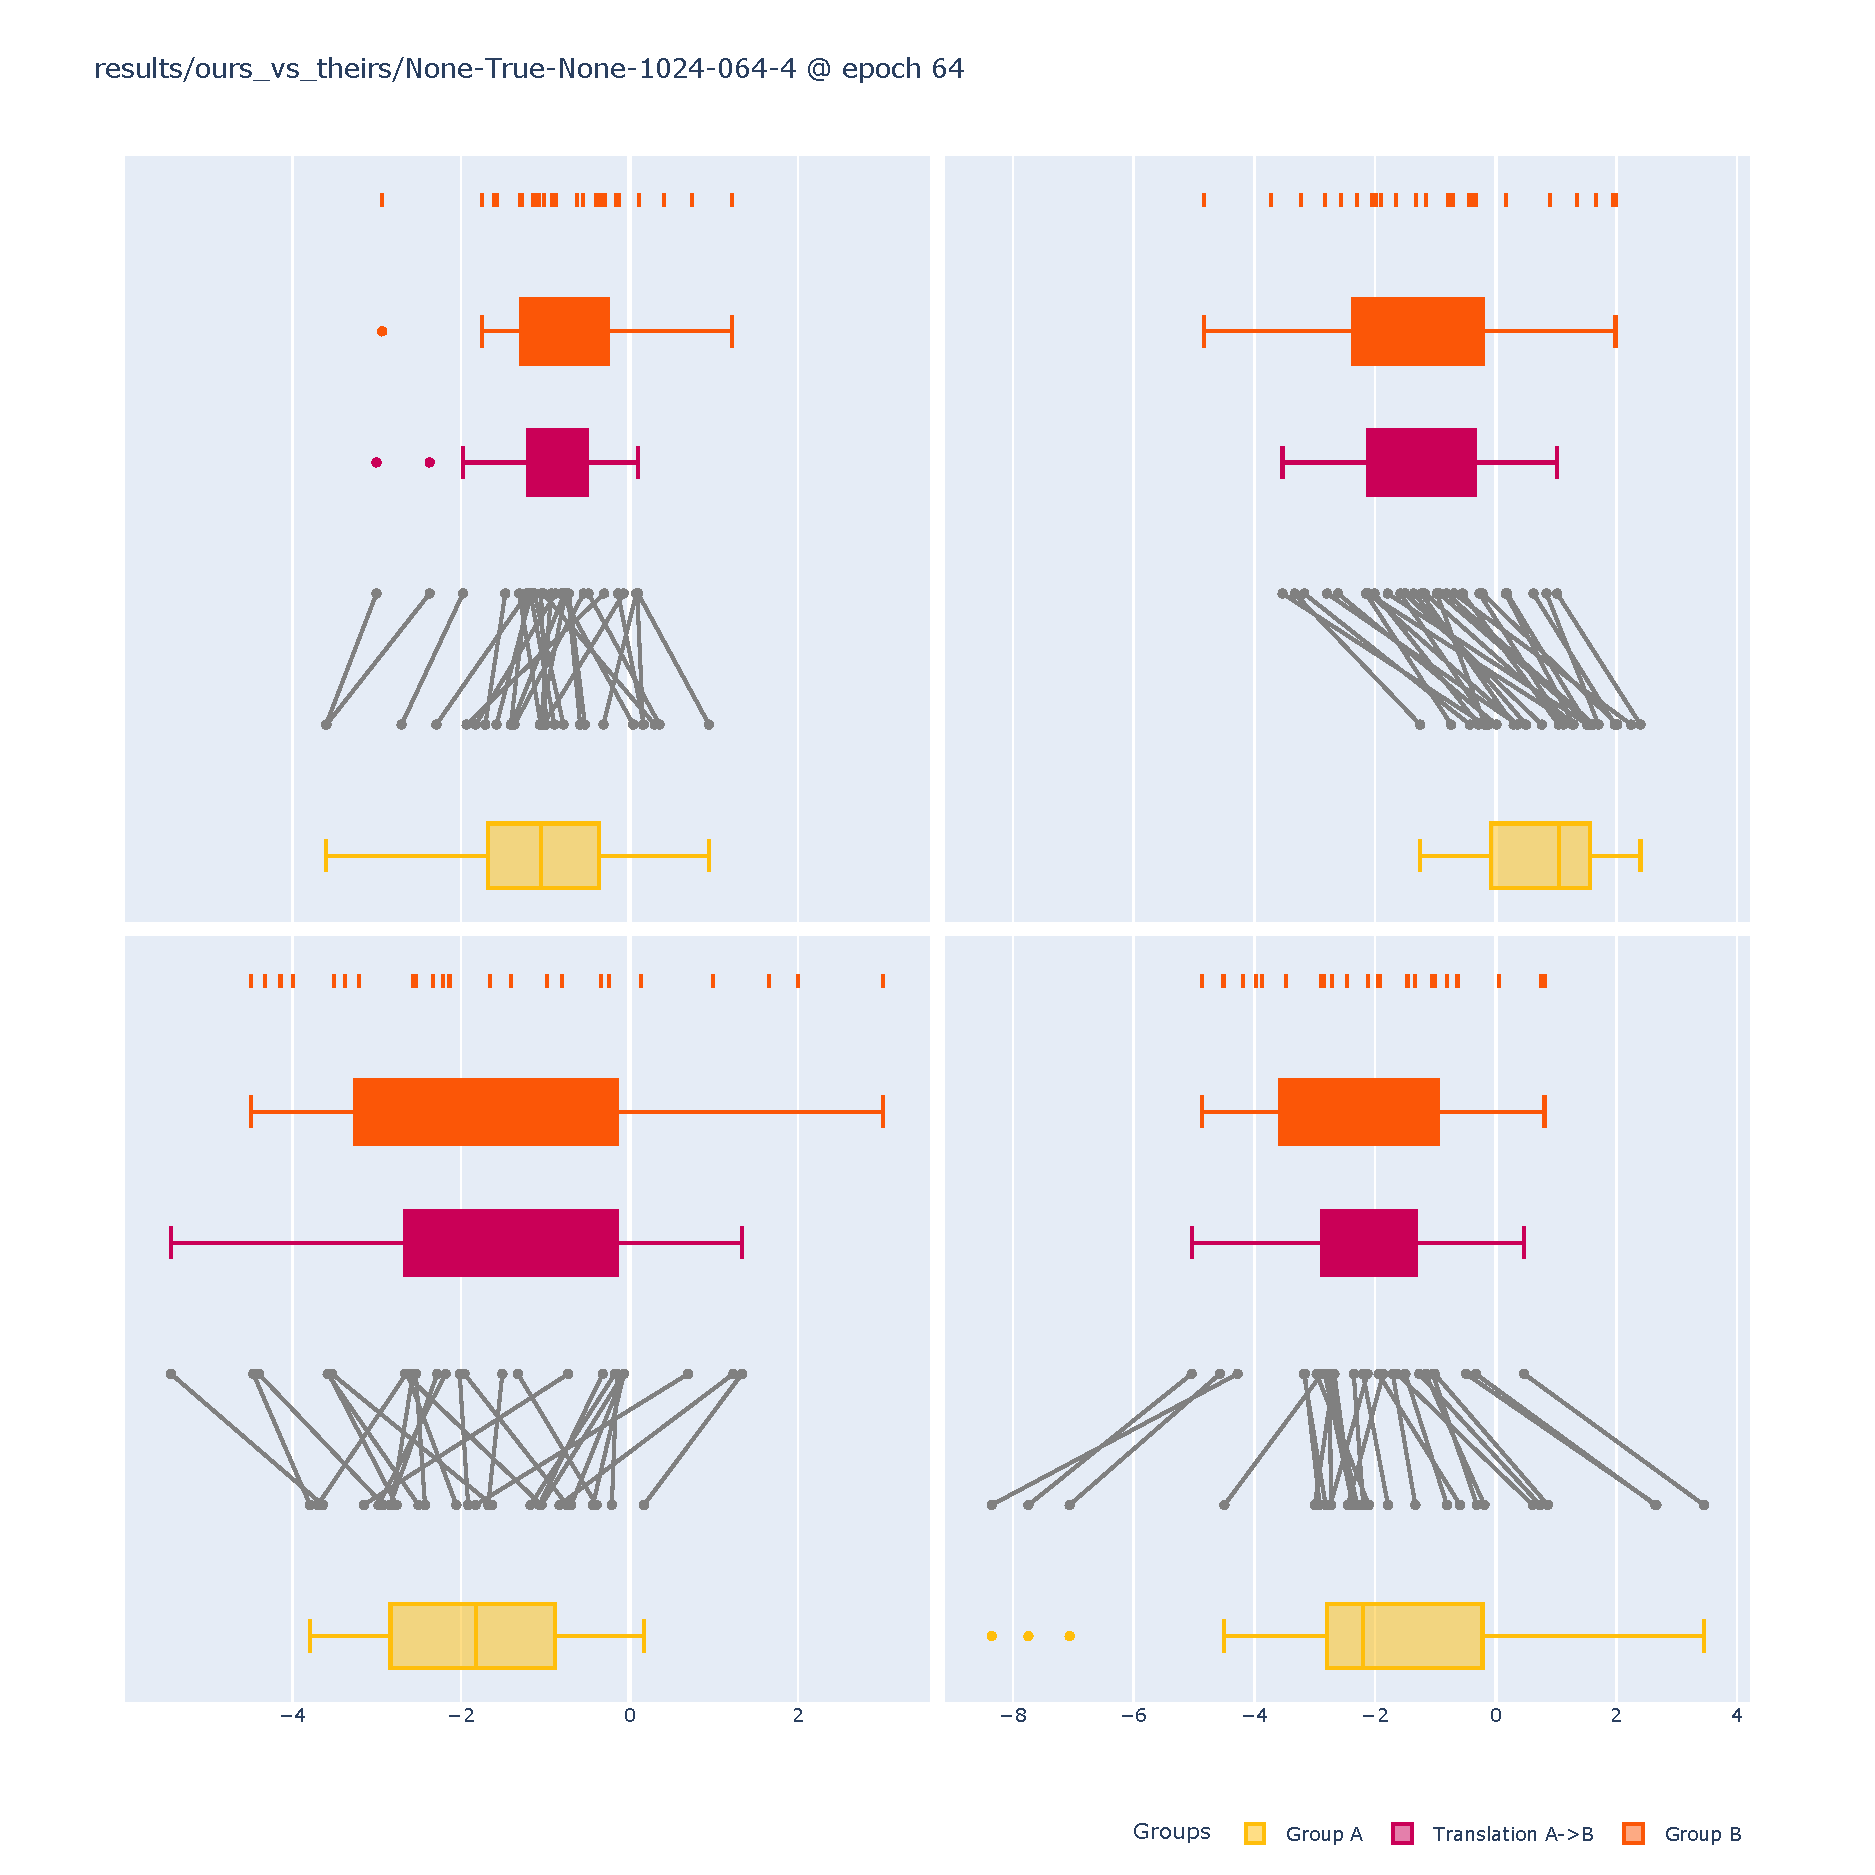
\includegraphics[width=\columnwidth]{files/ours.pdf}}
    \centerline{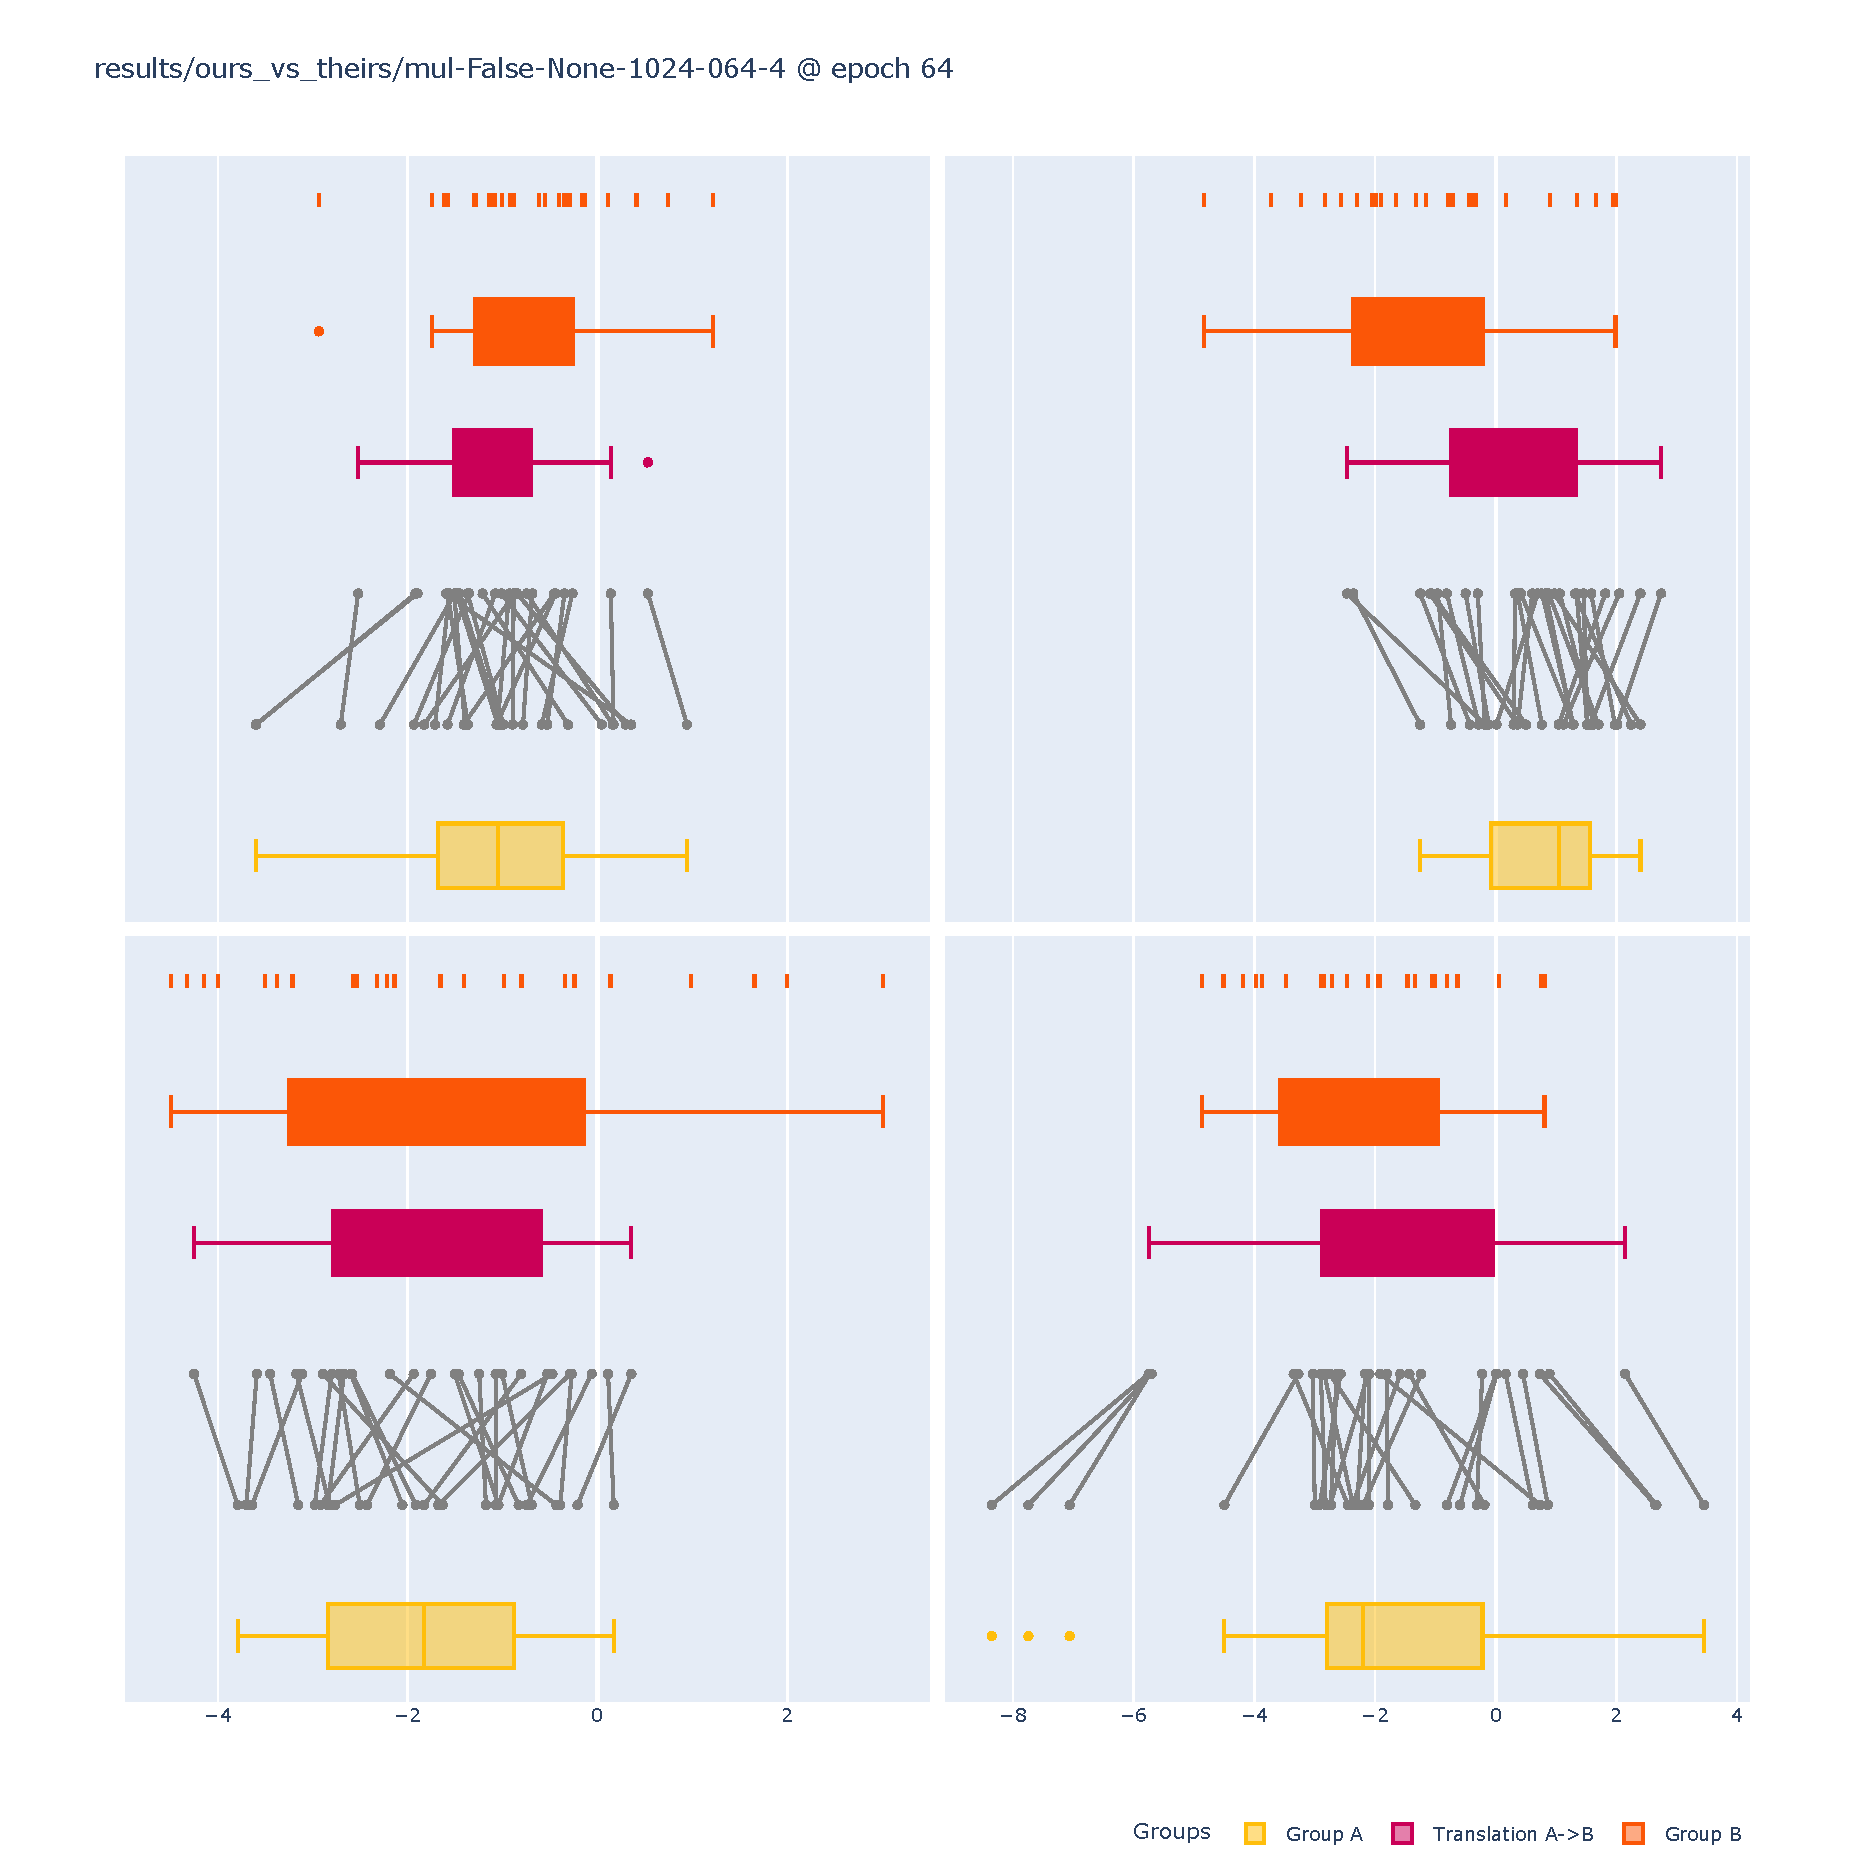
\includegraphics[width=\columnwidth]{files/theirs.pdf}}
    \caption{Qualitative comparison of unsupervised translation between CxVAE (top) and ML-VAE \citep{Bouchacourt2018MultiLevelVA} (bottom). Our model captures the distribution of values in the target group better than the existing methods.}
    \label{qualitative}
    \end{center}
    \vskip -0.2in
\end{figure}

We test CxVAE against the other models from the GVAE family.

\subsection{Quantitative Evaluation}

\begin{figure}[ht]
    \vskip 0.2in
    \begin{center}
    \centerline{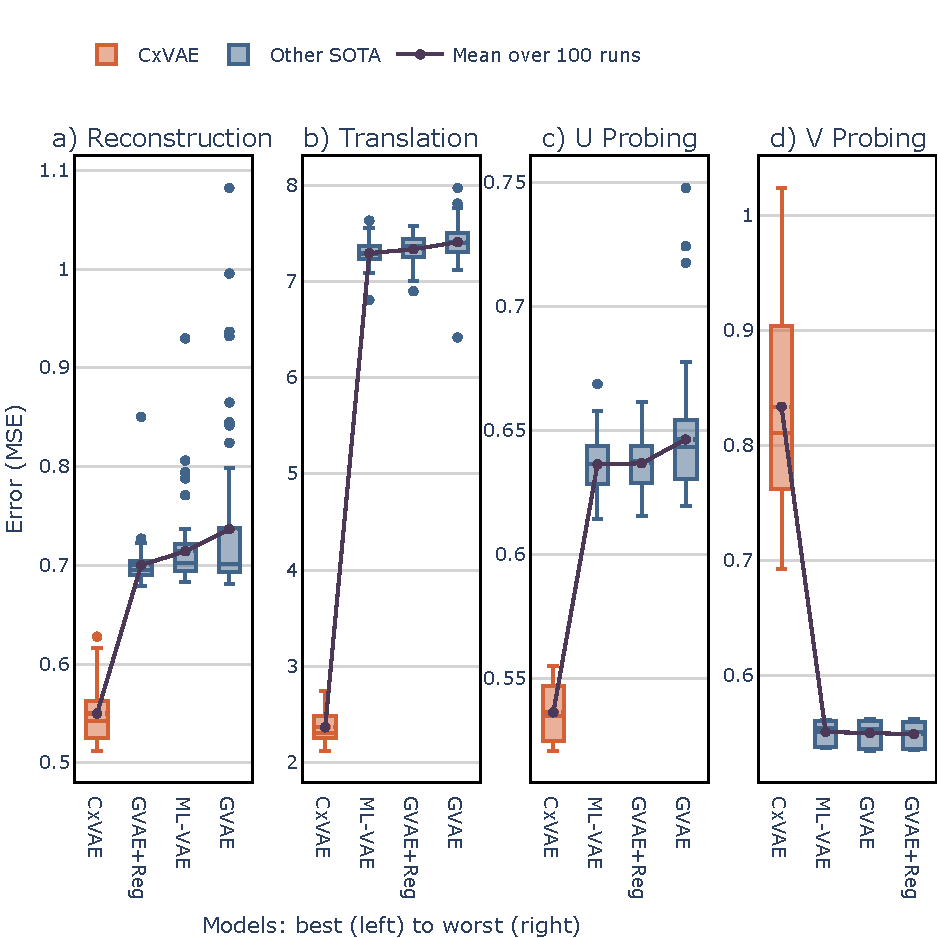
\includegraphics[width=\columnwidth]{files/results.pdf}}
    \caption{\textbf{Errors on the holdout set by training epoch.} We compare CxVAE (ours, yellow) with \citet{Bouchacourt2018MultiLevelVA} (purple), \citet{Hosoya2019GroupbasedLO} (orange), and
    \citet{Nmeth2020AdversarialDW} (red). For each model we perform 7 training runs, displaying the lowest, highest, and median error at each epoch.}
    \label{results}
    \end{center}
    \vskip -0.2in
\end{figure}


\begin{table*}[t]
    \caption{\textbf{Comparison between errors on the holdout set of our model (CxVAE) and the rest of the GVAE family.} CxVAE has the best performance across the 4 criteria. All errors are MSE, so lower is better. A mean error and standard deviation over the 7 training runs is taken at every epoch, and then the last 20 training epochs (44 - 64) are averaged in order to be displayed.}
    \label{results}
    \vskip 0.15in
    \begin{center}
    \begin{small}
    \begin{sc}
    \begin{tabular}{lcccc}
    \toprule
    Model & Rec Err & Trans Err & $u$-pred Err & $v$-pred Err \\
    \midrule
    CxVAE (ours) & \textbf{52.1} $\pm$ 0.6 & \textbf{219.5} $\pm$ 4.7 & \textbf{53.3} $\pm$ 1.2 & \textbf{30.2} $\pm$ 0.3 \\
    ML-VAE \citep{Bouchacourt2018MultiLevelVA} & 69.8 $\pm$ 1.6 & 738.8 $\pm$ 13.6  & 63.4 $\pm$ 1.0 & 63.0 $\pm$ 0.3 \\
    GVAE \citep{Hosoya2019GroupbasedLO} & 71.9 $\pm$ 4.3 & 742.9 $\pm$ 14.4 & 63.1 $\pm$ 0.9 & 63.0 $\pm$ 0.4 \\
    GVAE + Reg \citep{Nmeth2020AdversarialDW} & 70.0 $\pm$ 1.4 & 735.3 $\pm$ 13.0 & 63.8 $\pm$ 1.1 & 63.0 $\pm$ 0.5 \\
    \bottomrule
    \end{tabular}
    \end{sc}
    \end{small}
    \end{center}
    \vskip -0.1in
\end{table*}

\subsection{Ablation Study}

\begin{table*}[t]
    \caption{\textbf{Ablation study comparing CxVAE (our model) with alternative models obtained by replacing each of the novel components (group encoder, instance encoder and regularization).} Each replacement leads to a worse performance across all criteria.}
    \label{ablation}
    \vskip 0.15in
    \begin{center}
    \begin{small}
    \begin{sc}
    \begin{tabular}{lcccc}
    \toprule
    Model & Rec Err & Trans Err & $u$-pred Err & $v$-pred Err \\
    \midrule
    CxVAE (ours) & \textbf{52.1} $\pm$ 0.6 & \textbf{219.5} $\pm$ 4.7 & \textbf{53.3} $\pm$ 1.2 & \textbf{30.2} $\pm$ 0.3 \\ 
    \midrule \multicolumn{5}{c}{$u$ Encoder} \\ \midrule
    Average & 53.6 $\pm$ 2.2 & 224.7 $\pm$ 10.0 & 53.4 $\pm$ 1.1 & 30.9 $\pm$ 1.1 \\
    Multiplication & 54.9 $\pm$ 2.8 & 229.2 $\pm$ 7.8 & 53.4 $\pm$ 0.9 & 31.4 $\pm$ 1.0 \\ 
    \midrule \multicolumn{5}{c}{$v$ Encoder} \\ \midrule
    Unconditional & 72.3 $\pm$ 3.6 & 729.0 $\pm$ 15.1 & 63.6 $\pm$ 1.2 & 63.0 $\pm$ 0.3 \\
    \midrule \multicolumn{5}{c}{Regularization} \\ \midrule
    None & 54.1 $\pm$ 1.9 & 235.5 $\pm$ 16.5 & 53.6 $\pm$ 1.4 & 31.6 $\pm$ 1.5 \\
    Unconditional IB & 53.7 $\pm$ 1.2 & 225.7 $\pm$ 5.7 & 53.5 $\pm$ 1.1 & 30.8 $\pm$ 0.6 \\
    \bottomrule
    \end{tabular}
    \end{sc}
    \end{small}
    \end{center}
    \vskip -0.1in
\end{table*}

In order to quantify the effect of each proposed improvement, we perform an ablation study whereby we measure the decrease in performance resulting from replacing a proposed element of our model with a current alternative.

The proposed improvements have the best individual performance with respect to both reconstruction and translation error in each of the three categories. The choice of a group-aware instance encoder leads to the most significant increase in performance.

\bibliography{main}
\bibliographystyle{icml2022}


%%%%%%%%%%%%%%%%%%%%%%%%%%%%%%%%%%%%%%%%%%%%%%%%%%%%%%%%%%%%%%%%%%%%%%%%%%%%%%%
%%%%%%%%%%%%%%%%%%%%%%%%%%%%%%%%%%%%%%%%%%%%%%%%%%%%%%%%%%%%%%%%%%%%%%%%%%%%%%%
% APPENDIX
%%%%%%%%%%%%%%%%%%%%%%%%%%%%%%%%%%%%%%%%%%%%%%%%%%%%%%%%%%%%%%%%%%%%%%%%%%%%%%%
%%%%%%%%%%%%%%%%%%%%%%%%%%%%%%%%%%%%%%%%%%%%%%%%%%%%%%%%%%%%%%%%%%%%%%%%%%%%%%%
\newpage
\appendix
\onecolumn
\section{You \emph{can} have an appendix here.}

You can have as much text here as you want. The main body must be at most $8$ pages long.
For the final version, one more page can be added.
If you want, you can use an appendix like this one, even using the one-column format.
%%%%%%%%%%%%%%%%%%%%%%%%%%%%%%%%%%%%%%%%%%%%%%%%%%%%%%%%%%%%%%%%%%%%%%%%%%%%%%%
%%%%%%%%%%%%%%%%%%%%%%%%%%%%%%%%%%%%%%%%%%%%%%%%%%%%%%%%%%%%%%%%%%%%%%%%%%%%%%%


\end{document}


% This document was modified from the file originally made available by
% Pat Langley and Andrea Danyluk for ICML-2K. This version was created
% by Iain Murray in 2018, and modified by Alexandre Bouchard in
% 2019 and 2021 and by Csaba Szepesvari, Gang Niu and Sivan Sabato in 2022. 
% Previous contributors include Dan Roy, Lise Getoor and Tobias
% Scheffer, which was slightly modified from the 2010 version by
% Thorsten Joachims & Johannes Fuernkranz, slightly modified from the
% 2009 version by Kiri Wagstaff and Sam Roweis's 2008 version, which is
% slightly modified from Prasad Tadepalli's 2007 version which is a
% lightly changed version of the previous year's version by Andrew
% Moore, which was in turn edited from those of Kristian Kersting and
% Codrina Lauth. Alex Smola contributed to the algorithmic style files.
